\subsection{Biblioteca de capturare a evenimentelor}\label{library}
Aceasta este prima și cea mai importantă dintre componentele
proiectului. Pentru că această bibliotecă este încărcată direct în
programul clientului, este proiectată să fie atât portabilă cât și
performantă.

Pentru a maximiza portabilitatea, alegerea naturală de limbaj
pentru bibliotecă este C\cite{C}: pentru că limbajul are o interfață
binară standardizată de ISO și implementată de majoritatea
compilatoarelor folosite în industrie, împreună cu faptul că majoritatea
limbajelor de nivel înalt implementează
\textit{foreign-function-interface} cu C, aplicațiile pot beneficia de
această bibliotecă aproape indiferent de limbajul în care au fost
programate sau platforma pe care sunt executate.

Deși există variante mai bune pentru performanță cum ar fi C++ sau
\textit{assembly}, C este un limbaj suficient de eficient pentru a fi
cea mai bună alegere, luând în considerare avantajul copleșitor de
portabilitate.

\subsubsection{Interfață}\label{section:library-interface}
Pentru că această bibliotecă este una generică, interfața este
intenționat minimală: sunt expuse în mod public 3 funcții și 4
constante numerice. În limbajul C, interfața poate fi descrisă astfel:
\begin{lstlisting}[
        caption=Interfața bibliotecii pentru capturare de evenimente]
    void syan_capture_event(int event_type, void* object);

    void* syan_initialize_event(int event_type);
    void syan_finalize_event(void* event, void* object);

    enum {
      SA_EV_CREATE = 1 << 28,
      SA_EV_DESTROY = 1 << 29,
      SA_EV_THREAD = 1 << 30,
      SA_EV_THREAD_ON_CREATE = SA_EV_THREAD | SA_EV_CREATE,
    };
\end{lstlisting}
Această bibliotecă expune ca funcționalitate principală capturarea
evenimentelor, așa că interfața publică importantă este funcția
\lstinline{syan_capture_event}, care îndeplinește exact acest scop.
Toate celelalte componente ale interfeței expuse sunt pentru a trata
cazuri particulare mai complexe sau a standardiza tipuri de evenimente
pe care se bazează și programul \lstinline{SyncAnalysis}, și sunt
descrise mai jos. Exemplul principal de utilizare după care a fost
proiectată funcția \lstinline{syan_capture_event} se poate vedea în
Fragmentul de cod \ref{code:library-interface-example}.

\begin{lstlisting}[caption=Exemplul folosit în proiectarea interfeței,
                   label=code:library-interface-example]

    #define EVENT_MUTEX_BEFORE_LOCK 1331
    #define EVENT_MUTEX_AFTER_LOCK 1332

    pthread_mutex_t* m;
    void f() {
        syan_capture_event(EVENT_MUTEX_BEFORE_LOCK, m);
        pthread_mutex_lock(m);
        syan_capture_event(EVENT_MUTEX_AFTER_LOCK, m);
    }
\end{lstlisting}

Funcția este apelată cu 2 parametri, unul pentru tipul de eveniment
capturat și celălalt pentru identitatea obiectului țintă al
evenimentului. Astfel, în analiza post-mortem a unui program se poate
face o corelare între mai multe evenimente care au avut loc pe același
obiect țintă. Cum obiectele în limbajul C au în mod implicit o
identitate dată de adresa de memorie unde sunt stocate, este natural ca
parametrul care identifică obiectul să aibă tipul de date
\lstinline{void*}, care reprezintă în mod convențional o adresă oarecare
de memorie. Apare totuși o problemă: aceași adresă de memorie poate fi
refolosită de-a lungul execuției unui program, pentru a stoca mai multe
obiecte logice diferite (după dealocarea primului obiect, la alocarea
unui obiect nou se poate folosi aceași memorie; un exemplu comun este
segmentul de memorie stivă al programului). Pentru a evita confuzii
generate de această problemă, biblioteca expune două constante numerice
\lstinline{SA_EV_CREATE} și \lstinline{SA_EV_DESTROY}, ce acționează ca
\textit{biți indicatori} în tipul unui eveniment: dacă în scrierea în
baza 2 a tipului unui eveniment bitul \lstinline{SA_EV_CREATE}
(respectiv \lstinline{SA_EV_DESTROY}) este 1, evenimentul este
considerat unul care marchează crearea un obiect (respectiv distrugerea
unui obiect).

Această convenție este folosită și de către programul
\lstinline{SyncAnalysis}, care se folosește de aceste evenimente pentru
a reconstrui o bază de date de obiecte active în fiecare punct al
execuției programului client, a include evenimentul ce marchează
crearea unui obiect țintă în rapoarte și a elibera memorie după
distrugerea unui obiect. Astfel, este recomandat ca orice bibliotecă de
integrare să folosească acești indicatori pentru a captura evenimente ce
marchează crearea și distrugerea tuturor obiectelor de interes pentru
evenimentele capturate de respectiva bibliotecă:
\begin{lstlisting}
    enum {
        EVENT_MUTEX = 1u << 15,
        EVENT_MUTEX_CREATE = EVENT_MUTEX | SA_EV_CREATE,
        EVENT_MUTEX_DESTROY = EVENT_MUTEX | SA_EV_DESTROY,
    };
\end{lstlisting}

Fiecare eveniment capturat conține identitatea firului de execuție care
l-a capturat. Este util atunci să se raporteze câte un eveniment care
marchează crearea fiecărui fir de execuție, pentru a putea pune
evenimentele capturate de un anumit fir de execuție într-un context.
Astfel, biblioteca în sine când se încarcă capturează ca prim eveniment
unul care marchează crearea firului de execuție care a încărcat
biblioteca. Pentru că biblioteca raportează în interiorul său un
eveniment de creare de fir de execuție, aceasta stabilește un număr
\lstinline{SA_EV_THREAD_ON_CREATE} (se observă în interfață că acest
număr conține bitul \lstinline{SA_EV_CREATE}) care să reprezinte
evenimentele de acest tip. Orice bibliotecă de integrare trebuie să dea
același număr pentru argumentul \lstinline{event_type} când apelează
funcția \lstinline{syan_capture_event} pentru a raporta crearea unui fir
nou de execuție.

Cu experiența implementării bibliotecilor de integrare s-a observat că
atunci când se raportează crearea unui nou fir de execuție folosind
biblioteca \lstinline{pthread}, identitatea obiectului țintă
al evenimentului este cunoscută abia după ce a pornit noul fir de
execuție:
\begin{lstlisting}[caption=Capturare incorectă a creării unui fir de
                           execuție]
    pthread_t T;
    pthread_create(&T, nullptr, func, arg);
    syan_capture_event(SA_EV_THREAD_ON_CREATE, (void*)T);
\end{lstlisting}
Dacă evenimentul care marchează crearea firului de execuție \textit{T}
este capturat \textit{după} crearea lui \textit{T}, pot apărea
inconsistențe în analiza post-mortem: firul de execuție \textit{T} poate
începe să captureze evenimente, care pot ajunge să apară în fișierul de
evenimente înaintea evenimentului care marchează crearea lui \textit{T}.
Pentru a rezolva această situație, biblioteca expune celelalte două
funcții \lstinline{syan_initialize_event} și
\lstinline{syan_finalize_event} în interfața bibliotecii.  Funcția
\lstinline{syan_initialize_event} crează evenimentul și îi alocă locul
în fișierul de evenimente \textit{înainte} de crearea firului
\textit{T}. După crearea firului \textit{T}, evenimentul este doar
marcat ca fiind \textit{finalizat}, dar este scris în fișier ca și cum
în locul unde a fost mai înainte apelat
\lstinline{syan_initialize_event} ar fi fost apelat
\lstinline{syan_capture_event}, rezolvând problema ridicată mai devreme.
Exemplul de mai sus se repară astfel:
\begin{lstlisting}[caption=Capturare corectă a creerii unui fir de
                           execuție]
    pthread_t T;
    void* ev = syan_initialize_event(SA_EV_THREAD_ON_CREATE);
    pthread_create(&T, nullptr, func, arg);
    syan_finalize_event(ev, (void*)T);
\end{lstlisting}

Se observă acum că funcția \lstinline{syan_capture_event} are o
implementare evidentă pe baza celor două funcții nou introduse:
\begin{lstlisting}[caption=Implementarea funcției
                   \lstinline{syan_capture_event}]
    void syan_capture_event(int event_type, void* object) {
        void* ev = syan_initialize_event(event_type);
        syan_finalize_event(ev, object);
    }
\end{lstlisting}

\subsubsection{Structura unui eveniment}\label{section:event-structure}

Un eveniment capturat de bibliotecă are aceași structură indiferent de
tipul evenimentului sau de identitatea obiectului țintă al acestuia.
Aceasta a fost proiectată astfel încât mai multe evenimente să poată fi
stocate ușor și eficient într-o zonă continuă de memorie și serializate
în format binar pe disc. În codul sursă C al bibliotecii, structura ce
definește un eveniment se poate vedea în Fragmentul de cod
\ref{code:event-structure}.
\begin{lstlisting}[caption=Structura unui eveniment capturat,
                   label=code:event-structure, float, floatplacement=H]
    typedef struct {
        int32_t signature;
        int32_t event_type;
        int64_t timestamp;
        intptr_t thread_id;
        intptr_t object_id;
        intptr_t backtrace[12];
    } SyanEvent;
\end{lstlisting}

Ordinea și dimensiunea în biți a fiecărui câmp a fost aleasă astfel
încât pe platformele cele mai populare, unde arhitectura procesorului
este pe 64 de biți și astfel dimensiunea unui \lstinline{intptr_t} este
8 bytes, un eveniment să aibă dimensiunea exact 128 bytes, fără spațiu
irosit din cauze precum \textit{padding} sau \textit{alignment}. Această
dimensiune, fiind o putere a lui 2 ($2^7=128$) mai are un avantaj:
dimensiunea paginii de RAM este în general tot o putere de 2, de obicei
4096 ($2^{12}$), și astfel pe o pagină de memorie încap exact 32 de
evenimente. Această proprietate este exploatată în bibliotecă pentru a
obține viteze mari de serializare a evenimentelor în memorie, și mai
apoi pe disc.

Câmpul \lstinline{signature} este folosit intern pentru a împiedica
biblioteca din a scrie un eveniment pe disc înainte de apelarea funcției
\lstinline{syan_finalize_event} pentru acel eveniment. Aceasta nu va
scrie evenimentul pe disc până când nu citește în câmpul
\lstinline{signature} valoarea prestabilită 666013. Valoarea câmpului
este 0 după apelul la funcția \lstinline{syan_initialize_event}, dar
evenimentul este deja pus în coada de evenimente ce trebuie scrise pe
disc. Când este apelată funcția \lstinline{syan_finalize_event},
valoarea este schimbată în 666013, permițând bibliotecii să continue
scrierea evenimentelor din coadă pe disc.

Câmpurile \lstinline{event_type} și \lstinline{object_id} vor conține
valorile date ca parametri de către client când acesta apelează funcția
\lstinline{syan_capture_event}, sau respectiv funcțiile
\lstinline{syan_initialize_event} și \lstinline{syan_finalize_event}.

Câmpul \lstinline{timestamp} este o reprezentare pe 64 de biți al
numărului de nanosecunde scurse de la inițializarea bibliotecii până la
momentul capturării evenimentului. Fișierul DUMP (descris în secțiunea
\textbf{\ref{dump-file}}) conține în \textit{header} momentul de timp al
inițializării bibliotecii, astfel momentul real de timp când a avut loc
evenimentul poate fi reconstruit post-mortem cu precizie de nanosecundă,
iar stocarea numărului de nanosecunde pe 64 de biți permite capturarea
evenimentelor într-un program cu durată de viață până la 146 de ani,
suficient pentru orice scop practic.

Câmpul \lstinline{thread_id} conține identitatea firului de execuție ce
a capturat evenimentul. Acesta este obținut printr-un apel la funcția
\lstinline{pthread_self()}, descrisă în specificația POSIX pentru fire
de execuție portabile\cite{pthread}. Deși specificația nu precizează
dacă tipul de date returnat de \lstinline{pthread_self()}, anume
\lstinline{pthread_t}, poate fi stocat cu succes într-o variabilă cu
tipul de date \lstinline{intptr_t}, în practică toate implementările
bibliotecii \lstinline{pthread} pentru platformele pe care a fost
testată biblioteca implementează \lstinline{pthread_t} ca pe un
\textit{pointer} la structura de control a firului de execuție (iar
acest \textit{pointer} poate fi stocat, conform definiției tipului de
date \lstinline{intptr_t}).

Câmpul \lstinline{backtrace} conține adresele de întoarcere din stiva de
execuție. Acestea sunt utile pentru ca în analiza post mortem să se
poată reconstrui stiva de apeluri de funcții așa cum este descris în
secțiunea \textbf{\ref{stack-reconstruction}} și să se poată construi
rapoarte cât mai exacte despre condițiile în care s-a capturat un
eveniment. Modul cum sunt capturate aceste adrese este descris mai pe
larg în secțiunea \textbf{\ref{stack-unwinding}}.

\subsubsection{Stiva de execuție}\label{stack-unwinding}

După compilarea programelor în cod de asamblare, tot codul este
structurat în funcții. Când o funcție apelează o altă funcție, aceasta
trebuie să își stocheze valorile variabilelor locale în memorie și
trebuie să îi transmită funcției apelate adresa de memorie unde să
reîntoarcă controlul odată ce și-a terminat execuția. Zona de memorie
unde funcțiile stochează aceste informații se numește segmentul de stivă
al programului. Fiecare fir de execuție are propriul segment stivă,
independent de celelalte fire.

\begin{figure}[ht]
\centering
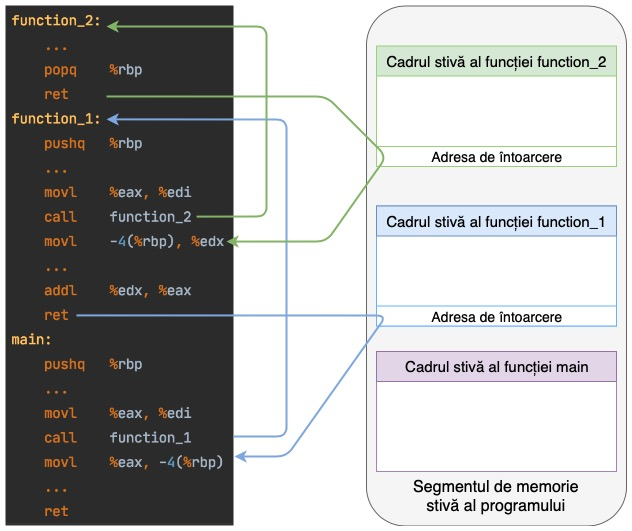
\includegraphics[width=14cm]{stack.jpg}
\caption{Stiva de execuție în arhitectura X86}
\label{fig:stack}
\end{figure}

În Figura \ref{fig:stack} se poate vedea acest procedeu pentru
arhitectura X86: în momentul apelului funcției \lstinline{function_1}
din funcția \lstinline{main}, se crează un nou cadru în memoria stivă a
programului (identificată pe desen prin culoarea albastru). La începutul
acestui cadru se stochează adresa de memorie a instrucțiunii următoare
apelului din funcția \lstinline{main}. În timpul execuției funcției
\lstinline{function_1}, aceasta apelează o a doua funcție
\lstinline{function_2}. Se crează deci un al treilea cadru în memoria
stivă (identificată pe desen prin culoarea verde), din nou stocându-se
adresa de întoarcere. La finalul funcției \lstinline{function_2},
aceasta invocă instrucțiunea \lstinline{ret}, care întoarce controlul la
adresa de memorie stocată în cadrul de stivă al funcției curente, adică
înapoi la funcția \lstinline{function_1}. Când și aceasta se termină
prin invocarea instrucțiunii ret, controlul este întors funcției
\lstinline{main}. Dacă aceasta nu mai este apelată la rândul său de
nicio altă funcție, instrucțiunea \lstinline{ret} de la sfârșitul
acesteia va încheia execuția programului, întorcând controlul sistemului
de operare.

A se observa că explicația dată mai sus nu descrie în mod exact cum
funcționează procesoarele și programele moderne, însă putem ajunge la
rezultate corecte pentru scopul nostru și fără a înțelege alte detalii
sau complicații istorice ale stivei de execuție. Singurul detaliu demn
de menționat este că în unele situații, compilatoarele de C și C++ pot
decide să \textit{optimizeze} programul prin omiterea stocării adresei
de întoarcere pe stivă, caz în care reconstruirea stivei de execuție
devine imposibilă. Pentru compilatorul Clang\cite{Clang}, această
optimizare poate fi oprită prin argumentul de compilare
\lstinline{-fno-omit-frame-pointer}.

Dacă funcția \lstinline{function_2} face un apel la funcția
\lstinline{syan_capture_event} pentru a captura un eveniment, vrem să
obținem lista de adrese de întoarcere din toate cadrele funcțiilor din
stivă. Acest rezultat poate fi obținut folosind biblioteca
\textit{libunwind}\cite{libunwind}, după cum se poate vedea în
Fragmentul de cod \ref{code:stack-unwinding}.

\begin{lstlisting}[caption=Capturarea stivei de execuție folosind
                           \lstinline{libunwind},
                   label=code:stack-unwinding,
                   float, floatplacement=H]
    #include <libunwind.h>
    void syan_get_backtrace(intptr_t* backtrace) {
        unw_context_t ctx;
        unw_getcontext(&ctx);
        unw_cursor_t crs;
        unw_init_local(&crs, &ctx);
        int n_frames = 0;
        while (n_frames < 12 && unw_step(&crs) > 0) {
            unw_word_t ip;
            if (unw_get_reg(&crs, UNW_REG_IP, &ip) < 0) break;
            backtrace[n_frames++] = (intptr_t)ip;
        }
    }
\end{lstlisting}

\subsubsection{Coada de evenimente și serializarea}\label{section:queue}

Am menționat deja mai devreme că un obiectiv în proiectarea acestei
biblioteci este ca performanța programului analizat să fie impactată cât
se poate de puțin. Trebuie luat în considerare astfel că scrierea
evenimentelor pe disc este o operațiune lentă. Prima decizie luată în
implementarea serializării este deci de a scrie evenimentele doar în
memoria RAM în cadrul firelor de execuție ale programului client, pentru
ca mai apoi un alt fir de execuție creat de bibliotecă să copieze datele
din memoria RAM pe disc. Pentru a obține rezultate satisfăcătoare de
performanță, am proiectat o \textit{coadă de evenimente} (intern numită
\lstinline{SyanBuffer}) specifică pentru această bibliotecă. Interfața
acestei cozi se poate vedea în Fragmentul de cod
\ref{code:queue-interface}.

\begin{lstlisting}[caption=Interfața cozii de evenimente folosite în
                           bibliotecă,
                   label=code:queue-interface, float, floatplacement=H]
#define SYAN_BUFFER_PAGE_SIZE 256
#define SYAN_BUFFER_NUM_PAGES 1024
typedef struct {
    SyanEvent storage[SYAN_BUFFER_PAGE_SIZE];
    int_fast32_t storage_front;
    atomic_int_fast32_t storage_back;
} SyanBufferPage;
typedef SyanBufferPage* SyanBufferPagePtr;
typedef struct {
    SyanBufferPagePtr pages[SYAN_BUFFER_NUM_PAGES];
    int_fast32_t pages_front;
    atomic_int_fast32_t pages_back;
} SyanBuffer;
int syan_buffer_init(SyanBuffer** b);
SyanEvent* syan_buffer_acquire_event_slot(SyanBuffer* b);
SyanBufferPagePtr syan_buffer_get_front_page(SyanBuffer* b);
void syan_buffer_release_front_page(SyanBuffer* b);
\end{lstlisting}
Prima proprietate importantă a acestei cozi este că nu conține niciun
mecanism explicit de sincronizare, ci doar câteva variabile cu tipul de
date \textit{atomic}. Minimizarea latenței punerii evenimentelor în
coadă este mai importantă decât eficiența citirii din coadă, pentru a
interfera cât mai puțin cu firele de execuție ale programului client.
Când un astfel de fir capturează un eveniment, memoria folosită pentru
a stoca informațiile acelui eveniment este direct memorie din câmpul
\lstinline{storage} al paginii curente din coadă (mai exact pagina
\lstinline{b->pages[b->pages_back]}). Asta omite necesitatea de a apela
funcții precum \lstinline{malloc} pentru a obține memorie pentru fiecare
eveniment individual sau \lstinline{memcpy} pentru a muta evenimentul
în coadă abia după ce acesta este complet format. Așadar funcția
\lstinline{syan_initialize_event} obține memoria necesară pentru
stocarea evenimentului apelând funcția
\lstinline{syan_buffer_acquire_event_slot}. Aceasta este implementată
folosind un algoritm \textit{lock-free} bazat pe operațiile de
\textit{compare-and-swap} și \textit{atomic-fetch-add} pe variabilele
atomice \lstinline{pages_back} și respectiv \lstinline{storage_back} din
acea pagină. Implementarea este similară cu cele descrise în articolele
\textit{Lock-free linked lists using compare-and-swap}
\cite{LinkedListsCAS} și
\textit{A practical nonblocking queue algorithm using compare-and-swap}
\cite{QueueCAS}.

După ce un eveniment a fost scris în coadă, acesta trebuie scris mai
departe pe disc. După cum am spus mai sus, biblioteca crează un fir de
execuție special pentru această operație. Fiind un singur fir care se
ocupă de scrierea pe disc a evenimentelor de la începutul cozii, se
poate observa și în interfață că variabilele \lstinline{pages_front} și
\lstinline{storage_front} nu sunt atomice: aceasta sunt atât scrise cât
și citite doar de firul intern al bibliotecii, așa că nu necesită
sincronizare. Am menționat și mai devreme cum un eveniment pus în coadă
nu este scris pe disc până când câmpul \lstinline{signature} al
evenimentului nu are valoarea corectă, scrisă de apelul funcției
\lstinline{syan_finalize_event}. În practică, firul de execuție al
bibliotecii citește aceste semnături din evenimentele de la începutul
cozii folosind operația \textit{atomic-load}, pentru că se așteaptă ca
scrierea să fie făcută de firul de execuție care raportează evenimentul.

Firul de execuție intern bibliotecii funcționează pe bază de iterații:
o iterație scrie cât de multe evenimente poate din coadă pe disc. Dacă
iterația a scris cu succes date pe disc, se trece direct la următoarea
iterație. Altfel, înseamnă că nu mai există evenimente noi capturate, și
firul apelează funcția de sistem \lstinline{usleep} pentru a permite
firelor programului client să își continue execuția înainte de a începe
o nouă iterație. Pentru a afla ce evenimente noi trebuie scrise pe disc,
firul verifică valorile câmpurilor \lstinline{storage_front} și
\lstinline{storage_back} de pe cea mai veche pagină a cozii, obținută
printr-un apel la funcția \lstinline{syan_buffer_get_front_page}. Dacă
valorile acestea sunt diferite, atunci toate evenimentele dintre sunt
fie evenimente noi capturate, fie evenimente în curs de capturare. Firul
așteaptă finalizarea tuturor acestor evenimente pe modelul
\textit{busy-wait}, deoarece se asumă că apelurile funcțiilor
\lstinline{syan_initialize_event} și \lstinline{syan_finalize_event}
se fac la puțin timp unul după celălalt. S-a experimentat aici și cu
alte modele de așteptare (\lstinline{pthread_sched_yield},
\lstinline{usleep}) și s-a observat empiric că \textit{busy-wait} se
comportă cel mai bine în practică. După ce toate aceste evenimente sunt
finalizate, ele sunt scrise împreună pe disc printr-un singur apel al
funcției standard C \lstinline{fwrite}. Dacă prin scrierea acestor
evenimente s-au scris toate evenimentele din pagină, aceasta este
eliberată. Altfel, se modifică doar câmpul \lstinline{storage_front} al
paginii pentru a marca până unde au fost scrise evenimentele din pagină.

\subsubsection{Fișiserului DUMP}\label{dump-file}

Am menționat în repetate rânduri că evenimentele capturate în timpul
execuției sunt scrise într-un fișier, denumit în continuare fișierul
DUMP. Dar acest fișier nu conține doar evenimentele, ci are și un antet
ce conține informații în plus despre execuție, utile pentru analiza
post-mortem a evenimentelor:
\begin{itemize}
    \item momentul când a fost inițializată biblioteca (o aproximare
    bună a momentului când a început execuția programului)
    \item calea către executabilul invocat
    \item argumentele din linia de comandă date executabilului
    \item adresa la care a fost încărcat executabilul
\end{itemize}

Momentul când a fost inițializată biblioteca este important pentru a
putea reconstrui momentul de timp când a fost capturat un eveniment,
pentru că valoarea câmpului \lstinline{timestamp} din fiecare eveniment
este egală cu numărul de nanosecunde ce au trecut între acest moment de
inițializare și momentul capturării evenimentului.

Calea către executabiul invocat și argumentelee din linia de comandă
sunt utile pentru a putea identifica ce reprezintă acest fișier DUMP. Nu
sunt folosite de către programul \lstinline{SyncAnalysis} decât pentru a
fi afișate în raportul de analizare.

Adresa de încărcare a executabilului este importantă pentru a putea
interpreta adresele din \lstinline{backtrace}-urile evenimentelor. Mai
multe detalii despre acest procedeu se găsesc în secțiunea 
\textbf{\ref{stack-reconstruction}}.

Fișierul DUMP este creat și deschis pentru scriere printr-un apel la
funcția standard C \lstinline{fopen("sync_analysis.dump", "wb")}.
Conform specificației acestei funcții, dacă un fișier cu același nume
exista deja, versiunea anterioară este ștearsă și un nou fișier gol este
creat oricum. Apelul la \lstinline{fopen} se face la inițializarea
bibliotecii, împreună cu scrierea antetului și pornirea firului intern
de execuție. În continuarea antetului sunt scrise direct evenimentele,
unul după celălalt, serializate în formatul binar descris în secțiunea
\textbf{\ref{section:event-structure}}.

\subsubsection{Măsurători de performanță}\label{library-performance}

Performanța bibliotecii se împarte în două metrici diferite: timpul
necesar capturării unui eveniment (metrica de \textit{latență}) și
volumul de evenimente ce poate fi serializat într-o perioadă de timp
(metrica de \textit{debit}). În Figurile \ref{fig:lib-perf-latency} și
\ref{fig:lib-perf-throughput} se pot vedea tabel cu măsurătorile
efectuate cu ajutorul bibliotecii
\lstinline{Google Benchmark}\cite{GoogleBenchmark} pentru ambele
metrici.

\begin{figure}[H]
\centering

\begin{center}
    \begin{tabular}{||c c||} 
        \hline
        Numărul firelor de execuție & Latența medie a capturării unui eveniment \\ [0.5ex] 
        \hline\hline
        1 & 569 ns \\ \hline
        2 & 601 ns \\ \hline
        3 & 615 ns \\ \hline
        4 & 670 ns \\ \hline
        5 & 811 ns \\ \hline
        6 & 1080 ns \\ \hline
    \end{tabular}
\end{center}

\caption{Măsurători de latență a bibliotecii}
\label{fig:lib-perf-latency}
\end{figure}

\begin{figure}[H]
\centering

\begin{center}
    \begin{tabular}{||c||} 
        \hline
        Debitul maxim pentru serializarea pe disc a evenimentelor \\ [0.5ex] 
        \hline\hline
        5'190'780 evenimente/secundă \\ \hline
    \end{tabular}
\end{center}

\caption{Măsurători de debit al bibliotecii}
\label{fig:lib-perf-throughput}
\end{figure}

Metrica de \textit{latență} este măsurată în \textit{nanosecunde} (cât
timp durează capturarea unui eveniment) și depinde de numărul de fire de
execuție ce capturează evenimente concurent, pentru că operațiile
\textit{compare-and-swap} implicate în acest procedeu au șansă mai mare
să eșueze cu cât sunt mai multe fire care încearcă să le execute în
același timp.

Metrica de \textit{debit} se măsoară în \textit{evenimente/secundă}
(câte evenimente pot fi serializate pe disc într-o perioadă de timp) și
nu depinde de nimic: aceasta reprezintă numărul \textit{maxim} de
evenimente a căror serializare poate fi cerută până când biblioteca nu
mai poate serializa evenimentele la viteza cu care vin acestea.

Măsurătorile au fost făcute pe o mașină Apple Macbook Pro, seria 2018,
cu procesorul Intel i7-8559U 2800MHz cu 4 nuclee fizice și 4 virtuale,
32KB L1 cache, 256KB L2 cache și 8MB L3 cache, cu memoria RAM 16 GB
2133 MHz LPDDR3 și disc SSD AP1024M.

Măsurătorile efectuate arată că biblioteca este într-adevăr eficientă în
capturarea evenimentelor și serializarea acestora: pe același sistem,
cererea de \textit{lock} pe un \textit{mutex} durează în medie 250ns
dacă există concurență de 4 fire de execuție care încearcă să dea
\textit{lock}. Capturarea a două evenimente care să marcheze cererea de
\textit{lock} (unul înainte și unul după această cerere) mai adaugă
1340ns la acest timp (536\% creștere pentru o astfel de operație).
Într-un experiment efectuat prin rularea programului
Chromium\cite{chromium} cu capturarea tuturor evenimentelor descrise în
\textbf{\ref{section:event-types}} (folosind biblioteca de integrare
\lstinline{syan_pthread_shim}, descrisă în Secțiunea
\textbf{\ref{section:pthread-shim}}), creșterea timpului de execuție
a programului în total a fost de 2.2\% (de la 6 minute și 3 secunde la 6
minute și 11 secunde pentru executarea testelor automate ale unui
proiect web).
